% !TEX root = ../main.tex

\chapter{{\sc adenine}: a HPC-oriented tool for biological data exploration} \label{chap:adenine}
% ADENINE

\begin{displayquote}
\textit{This chapter presents the first original contribution of the thesis, which is the 	 development of a machine learning framework designed for biological data exploration and visualization called \ade.
The goal of such framework is to help biomedical data scientists achieving a first and quick overview of the main structures underlying their data.
% researchers and data scientists
% and choosing the most suitable unsupervised learning pipeline for the problem at hand.
This software tool encompasses state of the art techniques for missing values imputing, data preprocessing, dimensionality reduction and clustering.
\ade has a scalable architecture which seamlessly work on single workstations as well as on high-performance computing facilities.
% \ade exploits both process- and thread-level parallelism and
\ade is capable of generating publication-ready plots along with quantitative descriptions of the results.
At the end of the chapter, few examples of exploratory analysis with \ade on biological datasets are presented.}
\end{displayquote}

%\ade is a machine learning framework designed for biological data exploration and visualization.
%Its goal is to help bioinformaticians achieving a first and quick overview of the main structures underlying their data.
%% researchers and data scientists
% % and choosing the most suitable unsupervised learning pipeline for the problem at hand.
%This software tool encompasses state-of-the-art techniques for missing values imputing, data preprocessing, dimensionality reduction and clustering.
%\ade has a scalable architecture which seamlessly work on single workstations as well as on high-performance computing facilities.
%% \ade exploits both process- and thread-level parallelism and
%\ade is capable of generating publication-ready plots along with quantitative descriptions of the results.
%In this paper we provide an example of exploratory analysis on a publicly available gene expression data set of colorectal cancer samples.
%The software and its documentation are available at  {\footnotesize \texttt{https://github.com/slipguru/adenine}} under FreeBSD license.

\section{Exploratory data analysis} \label{sec:data_exploration}

In biology, as well as in any other scientific domain, exploring and visualizing the collected measures is an insightful starting point for every data analysis process.
For instance, the aim of a biomedical study can be detecting groups of patients that respond differently to a given treatment, or inferring possible molecular relationships among all, or a subset, of the measured variables.
In both cases, data scientists will be asked to extract meaningful information from collections of complex and possibly high-dimensional measures, such as gene sequencing data, biomedical imaging, patients assessment questionnaires, and so on.

In these cases, a preliminary Exploratory Data Analysis (\ac{EDA}) is not only a good practice, but also fundamental before further and deeper investigations can take place.
To accomplish this task, several machine learning and data mining techniques were developed over the years (see Section~\ref{chap:state-of-the-art}).
Among those, we recall the combined use of the following classes of methods:
\begin{enumerate}
  \item missing values imputing;
  \item data preprocessing;
  \item dimensionality reduction;
  \item unsupervised clustering.
\end{enumerate}

Running EDA, despite being a valuable and widely applied data science practice, is definitely a nontrivial task.
For instance, given a dataset, it is usually unclear which algorithm will provide the most insightful results. A common practice is to empirically test some of them and compare their results from a qualitative/quantitative standpoint.
Moreover, applying EDA methods on large-scale data can be burdensome or even computationally unfeasible.

%\section{Popular data exploration tools} \label{sec:data_exploration_tools}

In the last few years, a fair number of data exploration software and libraries were released. Such tools may be grouped in two families: \ac{GUI}-based and command-line applications.
Among the first group we recall \text{Divvy} \cite{lewis2013divvy}, a software tool that performs dimensionality reduction and clustering on input data sets. \emph{Divvy} is a light framework; however,
its collection of {C/C++} algorithm implementations does not cover common strategies such as kernel principal component analysis \cite{scholkopf1997kernel} or hierarchical clustering \cite{hastie2009elements} and it does not offer strategies to perform automatic discovery of the number of clusters.
The most notable project that spans between the two families is \emph{Orange} \cite{demvsar2013orange}, a data mining software suite that offers both visual programming front-end and Python \ac{API}s. In the context of data exploration, \emph{Orange} can be successfully employed. However, in order to test different data analysis pipelines, each one must be manually created as it does not support their automatic generation.
Moreover, large data sets are difficult to analyze with both \emph{Divvy} and \emph{Orange} as they can run only on a single workstation, lacking of distributed computing support.

\section{\ade overview} \label{sec:adenine_overview}

\begin{table}[h!]
  \footnotesize
% \begin{longtable}{|>{\bfseries}l|>{\bfseries}l|>{\bfseries}l}
    \centering
    \begin{tabular}{lll}
        \toprule
        \bfseries Step &   \bfseries Algorithm & \bfseries Reference\\

        \multirow{2}{*}{Imputing} & mean &  \\
        & median & \\
        & most frequent & \\
        & $k$-nearest neighbors & \cite{troyanskaya2001missing} \\
        \midrule

        \multirow{4}{*}{Preprocessing} & recentering &  \\
        & standardize &  \\
        & normalize &  \\
        & min-max &  \\
        \midrule

        \multirow{9}{*}{\begin{tabular}{@{}c@{}}Dimensionality \\ reduction\end{tabular}} & principal component analysis (PCA)& \cite{jolliffe2002principal} \\
        & incremental PCA & \cite{ross2008incremental} \\
        & randomized PCA & \cite{halko2011finding} \\
        & kernel PCA & \cite{scholkopf1997kernel} \\
        & isomap & \cite{tenenbaum2000global} \\
        & locally linear embedding & \cite{roweis2000nonlinear} \\
        & spectral embedding & \cite{ng2002spectral} \\
        & multi-dimensional scaling & \cite{borg2005modern} \\
        & \begin{tabular}{@{}l@{}}t-distributed stochastic \\ neighbor embedding \end{tabular}   & \cite{van2008visualizing} \\
        \midrule

        \multirow{5}{*}{Clustering} & $k$-means &  \cite{bishop2006pattern}\\
        & affinity propagation & \cite{frey2007clustering} \\
        & mean shift & \cite{comaniciu2002mean} \\
        & spectral & \cite{shi2000normalized} \\
        & hierarchical & \cite{hastie2009elements} \\
        & DBSCAN & \cite{ester1996density} \\
        \bottomrule
    \end{tabular}
    \caption{Pipeline building blocks available in \ade.}\label{tab:blocks}
\end{table}


This chapter describes \ade, a command-line Python tool for biological data exploration and visualization that, combining different EDA methods, creates textual and graphical analytical reports of large scale, data collections.
%of an arbitrary number of pipelines.

Missing data imputing, preprocessing, dimensionality reduction and clustering strategies are considered as building blocks for constructing data analysis pipelines (see Section~\ref{sec:adenine_implementation}). The user is simply required to specify the input data and to select the desired blocks. \ade, then, takes care of generating and running the pipelines obtained by all possible combinations of the selected blocks. Every algorithm implementation of the presented software tool is inherited, or extended, from \sklearn \cite{scikit-learn} which is, to the best of our knowledge, the most complete machine learning open source Python library available online.

\ade natively supports data integration with the NCBI Gene Expression Omnibus (GEO) archive~\cite{barrett2013ncbi}, which data sets can be retrieved specifying their GEO accession number.

Thanks to its scalable architecture, \ade pipelines can seamlessly run in parallel as separate Python processes on single workstations or MPI\footnote{\url{http://mpi-forum.org/}} tasks in high-performance computing (HPC) cluster facilities. This remarkable feature allows to explore and visualize massive amounts of data in a reasonable computational time.
% \ade pipelines are designed to be independent from each other, therefore they all run in parallel as separate Python processes on different cores/machines.
Moreover, as \ade makes large use of {\sc numpy} and {\sc scipy}, it automatically benefits from their bindings with optimized linear algebra libraries (such as OpenBLAS or Intel\textsuperscript{\textregistered}~MKL).

\section{\ade implementation} \label{sec:adenine_implementation}
\ade is developed around the data analysis concept of \emph{pipeline}. A pipeline is a sequence of the following fundamental steps:
\begin{enumerate}
  \item missing values imputing;
  \item data preprocessing;
  \item dimensionality reduction and
  \item unsupervised clustering.
\end{enumerate}
For each task, different off-the-shelf algorithms can be used (see Table~\ref{tab:blocks}).

Data collected in biomedical research studies often present missing values.
Devising imputing strategies is a common practice~\cite{de2015impact} to deal with such issue.
\ade offers an improved version of the {\footnotesize \texttt{Imputer}} class provided by {\sc scikit-learn}. In addition to the pre-existent feature-wise \emph{mean}, \emph{median} and \emph{most frequent} strategies, this extension presents the $k$-nearest neighbors imputing method proposed for microarray data in~\cite{troyanskaya2001missing}.

% \ade presents different data preprocessing strategies to tackle undesired effects that may arise from heterogeneous measures possibly lying in very different numerical range.
 % when dealing with data collected from heterogeneous sources.
Collecting data from heterogeneous sources may imply dealing with variables lying in very different numerical ranges and this could have a negative influence on the behavior of data analysis techniques. To tackle this issue \ade offers different strategies to preprocess data, such as re-centering, standardizing or rescaling.

The presented software includes a set of linear and nonlinear dimensionality reduction and manifold learning algorithms that are particularly suited for exploration and visualization of high-dimensional data. Such techniques rely on the fact that it is often possible to \emph{decrease} the dimensionality of the problem estimating a low-dimensional embedding in which the data lie.

Besides offering a wide range of clustering techniques,
\ade implements strategies and heuristics to automatically estimate parameters that yield the most suitable cluster separation.
The optimal parameter selection of centroid-based algorithms follows the $B$-fold cross-validation strategy presented in Algorithm~\ref{alg:clusters}, where $\mathcal{S}(X,y)$ is the mean silhouette coefficient \cite{rousseeuw1987silhouettes} for all input samples.

\begin{algorithm}[]
  \caption{Automatic discovery of the optimal clustering parameter.}\label{alg:clusters}
    \begin{algorithmic}[1]
        \For{clustering parameter $k$ in $k_1 \dots k_K$ }
        \For{cross-validation split $b$ in $1 \dots B$}
              \State $X^{tr}_b,X^{vld}_b\leftarrow$ $b$-th training, validation set
              \State $\hat{m}\leftarrow$ fit model on $X^{tr}_b$
              \State $\hat{y}\leftarrow$ predict labels of $X^{vld}_b$ according to $\hat{m}$
              \State $s_b\leftarrow$ evaluate silhouette score  $\mathcal{S}(X^{vld}_b,\hat{y})$
        \EndFor
        \State $\bar{S}_k = \frac{1}{B}\sum_{i=1}^B s_i$
        \EndFor
        \State $k_{opt} = \argmax{k}(\bar{S}_k)$
    \end{algorithmic}
\end{algorithm}

For affinity propagation \cite{frey2007clustering} and $k$-means \cite{bishop2006pattern} clustering parameters can be automatically defined (\emph{preference} and \emph{number of clusters}, respectively).
% Clustering parameters for affinity propagation \cite{frey2007clustering} and k-means \cite{bishop2006pattern}, that are \emph{preference} and \emph{number of clusters}, can be automatically defined.
Mean shift~\cite{comaniciu2002mean} and DBSCAN~\cite{ester1996density} offer an implicit cluster discovery.
For hierarchical~\cite{hastie2009elements} and spectral clustering~\cite{shi2000normalized}, no automatic discovery of clustering parameters is offered. However, graphical aids are generated to evaluate clustering performance such as dendrogram tree and eigenvalues of the Laplacian of the affinity matrix plots, respectively.
% \todo{@fede DBSCAN}

\todo{more on hpc stuff}

\section{Usage example} \label{sec:usage_example}
In this section we show how \ade can be used to perform two EDAs on a gene expression microarray data set obtained from the GEO repository (accession number GSE87211).
This data set was collected in a recent medical study that aimed at understanding the underlying mechanism of colorectal cancer (CRC) as well as identifying molecular biomarkers, fundamental for the disease prognostication.
It is composed of $203$ colorectal cancer samples and $160$ matched mucosa controls. The adopted platform was the Agilent-026652 Whole Human Genome Microarray, which was used to measure the expression of $34127$ probe sets.

\ade offers a handy tool to automatically download the data set from the GEO repository given only its accession name.
It also let the user select phenotypes and/or probe sets of interest. Given these preferences, \ade automatically converts the data set from the \textit{SOFT} format to a comma-separated values text file. To download the remote GEO data set specifying the tissue type as phenotype of interest we used the following command.

{\footnotesize
\begin{lstlisting}[language=bash,caption={ }]
$ ade_GEO2csv.py GSE87211 --label_field characteristics_ch1.3.tissue
\end{lstlisting}
}

\noindent This automatically creates \texttt{{\footnotesize GSE87211\_data.csv}} and \texttt{{\footnotesize GSE87211\_labels.csv}} which contain gene expression levels and tissue type of each sample, respectively.

The first EDA aims at stratifying the samples according to their tissue type (mucosa or rectal tumor) this can be performed by executing the following command.

{\footnotesize
\begin{lstlisting}[language=bash,caption={ }]
$ ade_run.py ade_config.py
\end{lstlisting}
}

\noindent Where \texttt{{\footnotesize ade\_config.py}} is a configuration file which should look like the snippet below.

\todo{config here}

% Figure~\ref{fig:scatter} shows one of several possible comparisons between three pipelines on an RNA-Seq gene expression data set available both on UCI Machine Learning Repository and \ade documentation webpage.
% First \ade is installed via the Python Package Index, then

\noindent Each \texttt{step} variable refers to a dictionary having the name of the building block as key and a list as value. Each list has a \emph{on$\backslash$off} trigger in first position followed by a dictionary of keyword arguments for the class implementing the corresponding method. When more than one method is specified in a single step, or more than a single parameter is passed as {list}, \ade generates the pipelines composed of all possible combinations.

The configuration snippet above generates eight pipelines with similar structure. The first and the second halves have recentered and $\ell_2$-normalized samples, respectively. Each sample is then projected on a 2D space by isomap or by linear, Gaussian or polynomial kernel PCA. $k$-means clustering with automatic cluster discovery is eventually performed on each dimensionality-reduced data set, as in Algorithm~\ref{alg:clusters}.
Results of such pipelines are all stored in a single output folder. Once this process is completed, plots and reports can be automatically generated running the following command.

{\footnotesize
\begin{lstlisting}[language=bash,caption={ }]
  $ ade_analysis.py results/ade_output_folder_YYYY-MM-DD_hh:mm:ss
\end{lstlisting}
}

 % \texttt{ade\_analysis.py} with the output folder previously created as the only input argument.
% Data-points and backgrounds are colored as real classes and clustering predictions.

The aim of the second EDA is to uncover the relationships among a set of genes known from the literature to be strongly associated with CRC. Specifically this signature is composed of the following genes: \apc, \kras, \ctnnb, \tp, \msh, \mlh, \pms, \pten, \smad, \stk, \gsk and \axin~\cite{schulz2005molecular}.
We also considered probe sets measuring expression level of the same gene, and we labelled them with a progressive number.
%We also considered all the available gene isoforms, labelled with a progressive number.
Three partially overlapping sublists compose this signature.
\begin{enumerate}
  \item[\emph{S1)}] Genes fundamental for the progression of CRC (\ie~\apc, \kras, \ctnnb, \tp).
  \item[\emph{S2)}] Genes relevant in the \textit{Wnt signaling pathway}, which is strongly activated in the first phases of CRC (\ie~\apc, \ctnnb, \gsk, \axin).
  \item[\emph{S3)}] Genes involved in hereditary syndromes which predispose to CRC (\ie~\apc, \msh, \mlh, \pms, \pten, \smad, \stk)~\cite{schulz2005molecular}.
\end{enumerate}

A reduced version of the GEO data set that comprises only such genes can be easily created calling \texttt{{\footnotesize ade\_GEO2csv.py}} with the option \texttt{{\footnotesize -{}-signature GENE\_1,GENE\_2,...,GENE\_N}}. On the same line, the option \texttt{{\footnotesize -{}-phenotypes P\_1,P\_2,...,P\_M}} can be used to keep only mucosa or rectal tumor samples.
To run such experiment, one simply needs to select and activate the hierarchical clustering building block and to follow the same steps presented above.
% procedures that are similar to the one described above can be followed.


For \ade installation instructions and for a comprehensive description of all the options available in the configuration file we refer to the online documentation and tutorials\footnote{\url{http://slipguru.github.io/adenine}}.

\section{Results} \label{sec:results}

In the first EDA, we compared the clustering performance achieved by the eight \ade pipelines and we reported in Figure~\ref{fig:scatter} an intuitive visualization of the results achieved by the top three, evaluated in terms of silhouette score~\cite{rousseeuw1987silhouettes}. As expected, the top performing pipelines show a clear separation between the two sample groups, as the $k$-means algorithm devises a domain partitioning that is consistent with the actual tissue types.

\begin{figure}[!ht]
    \centering
    \subfloat[]{%
        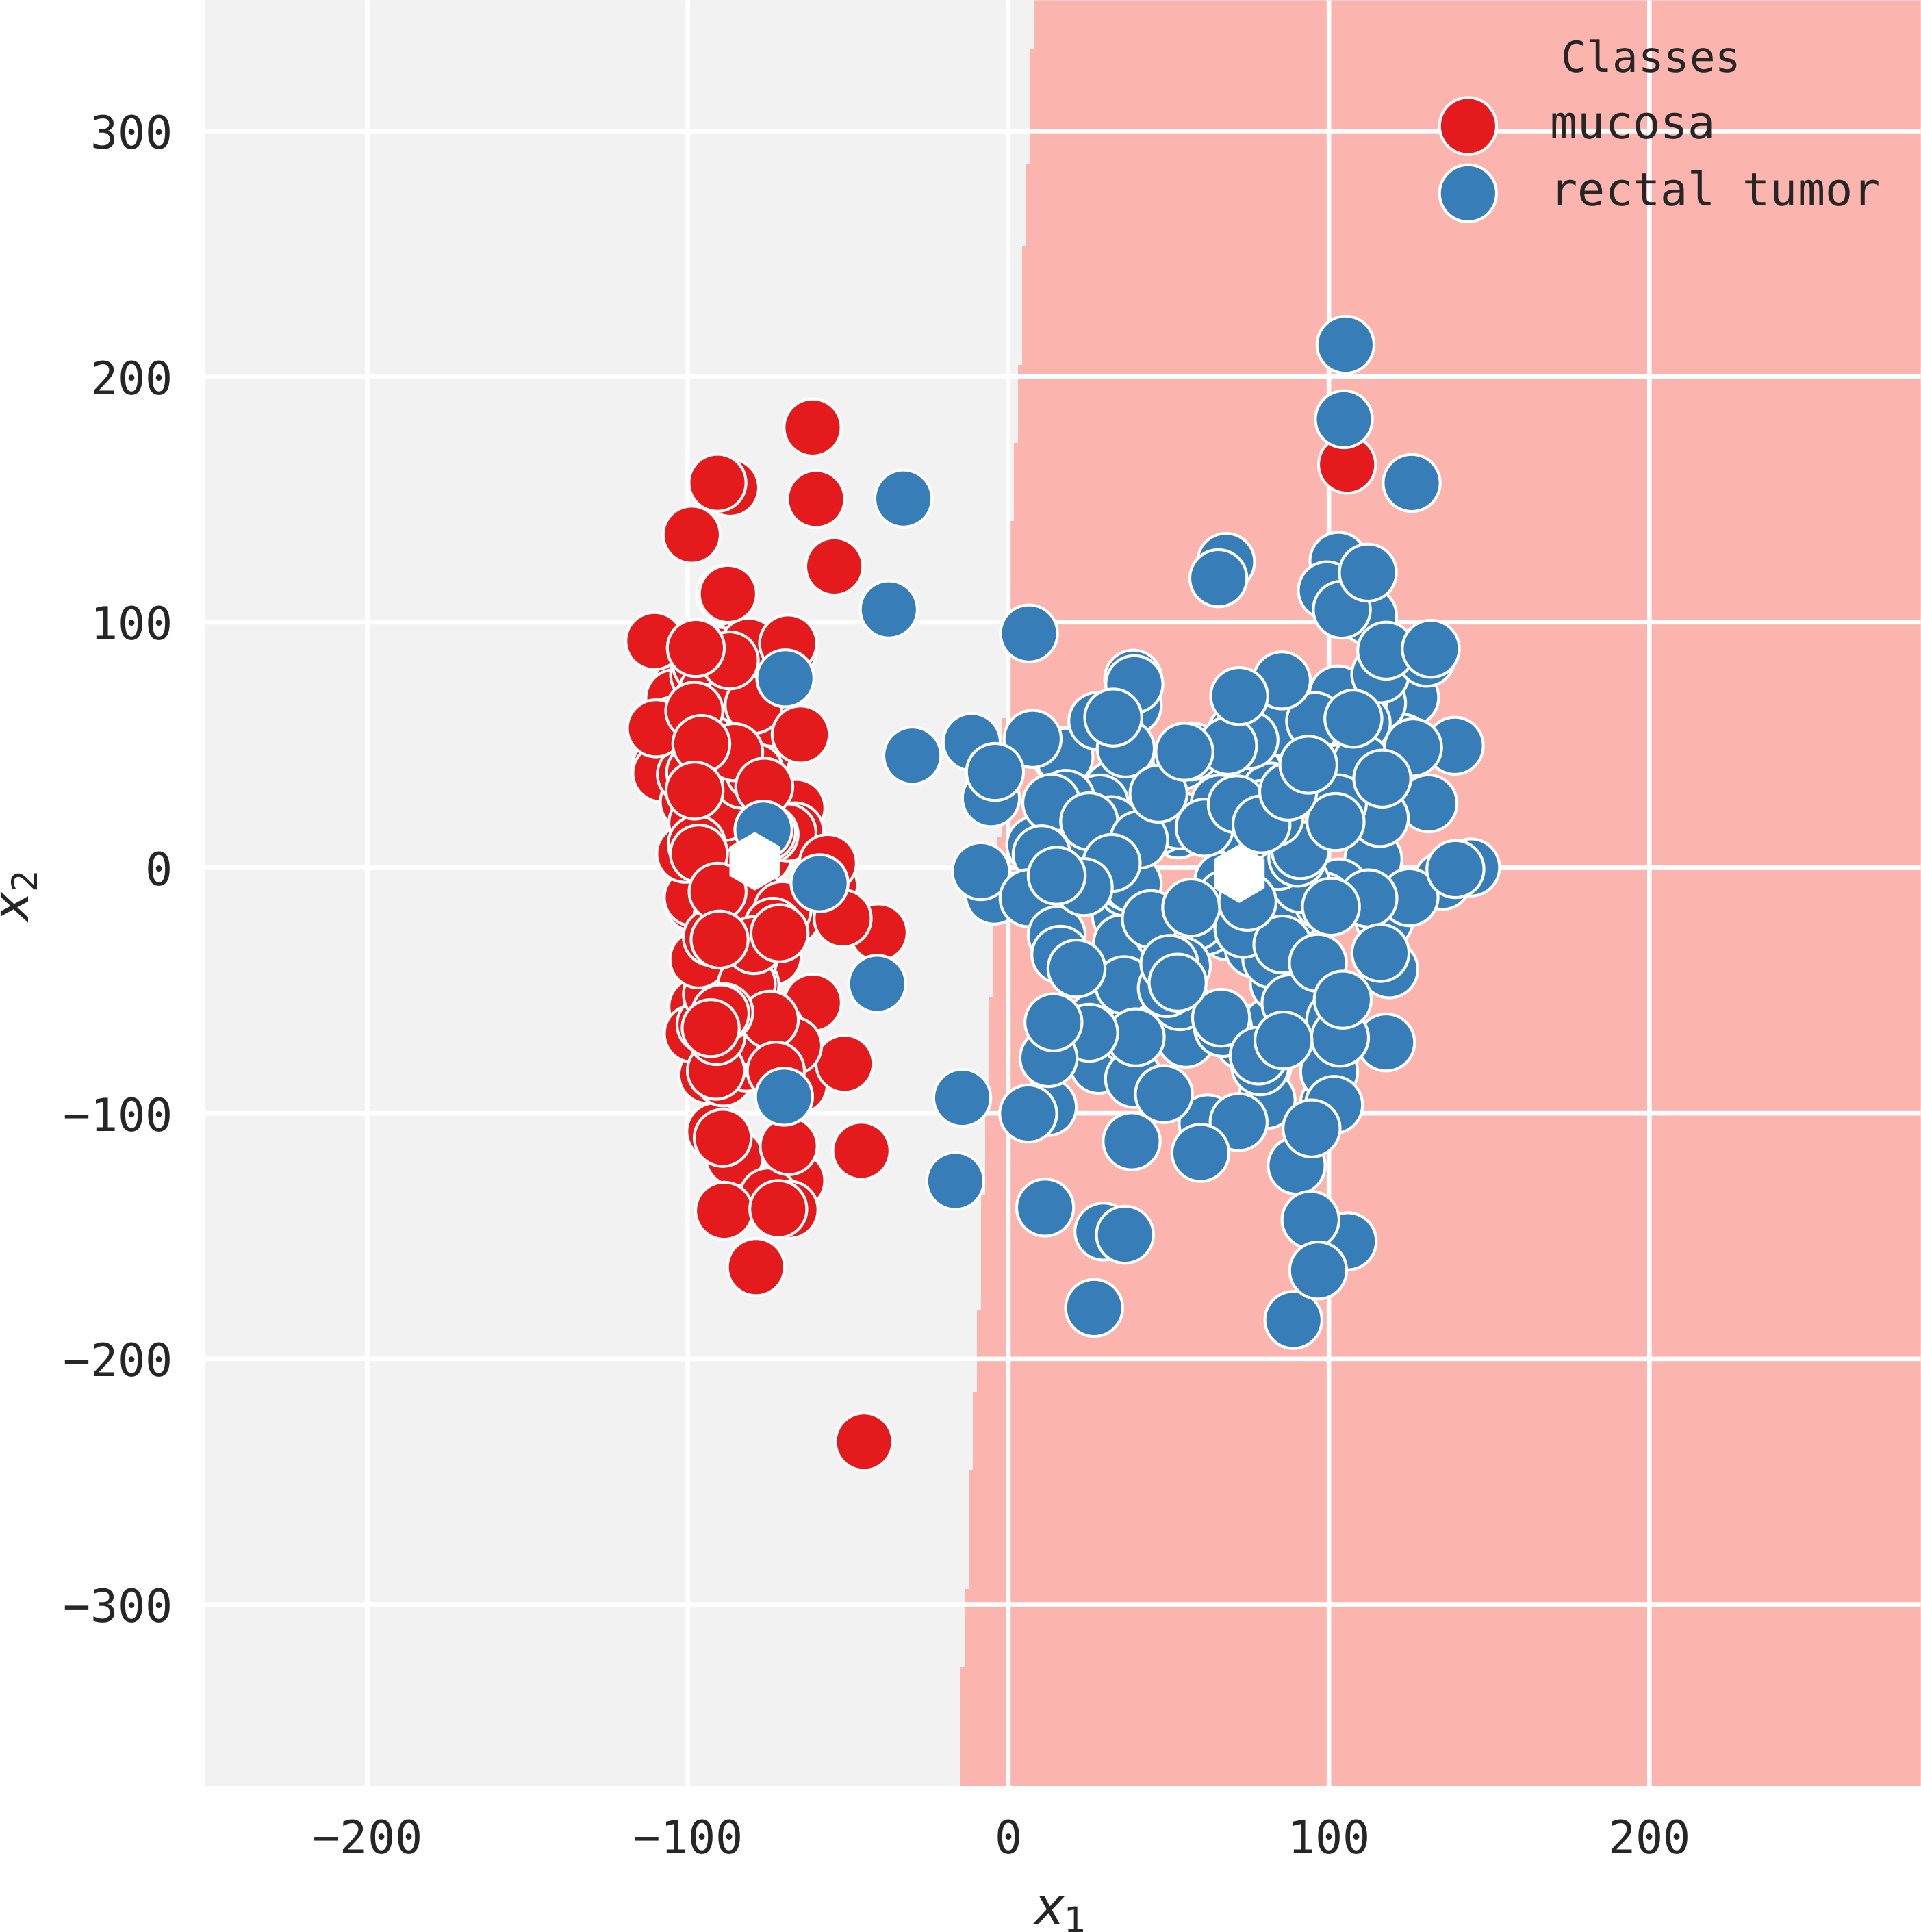
\includegraphics[width=0.32\textwidth]{part2/KMeans_2-clusts_linear.png}
        \label{fig:a}%
    }%
    \hfill%
    \subfloat[]{%
        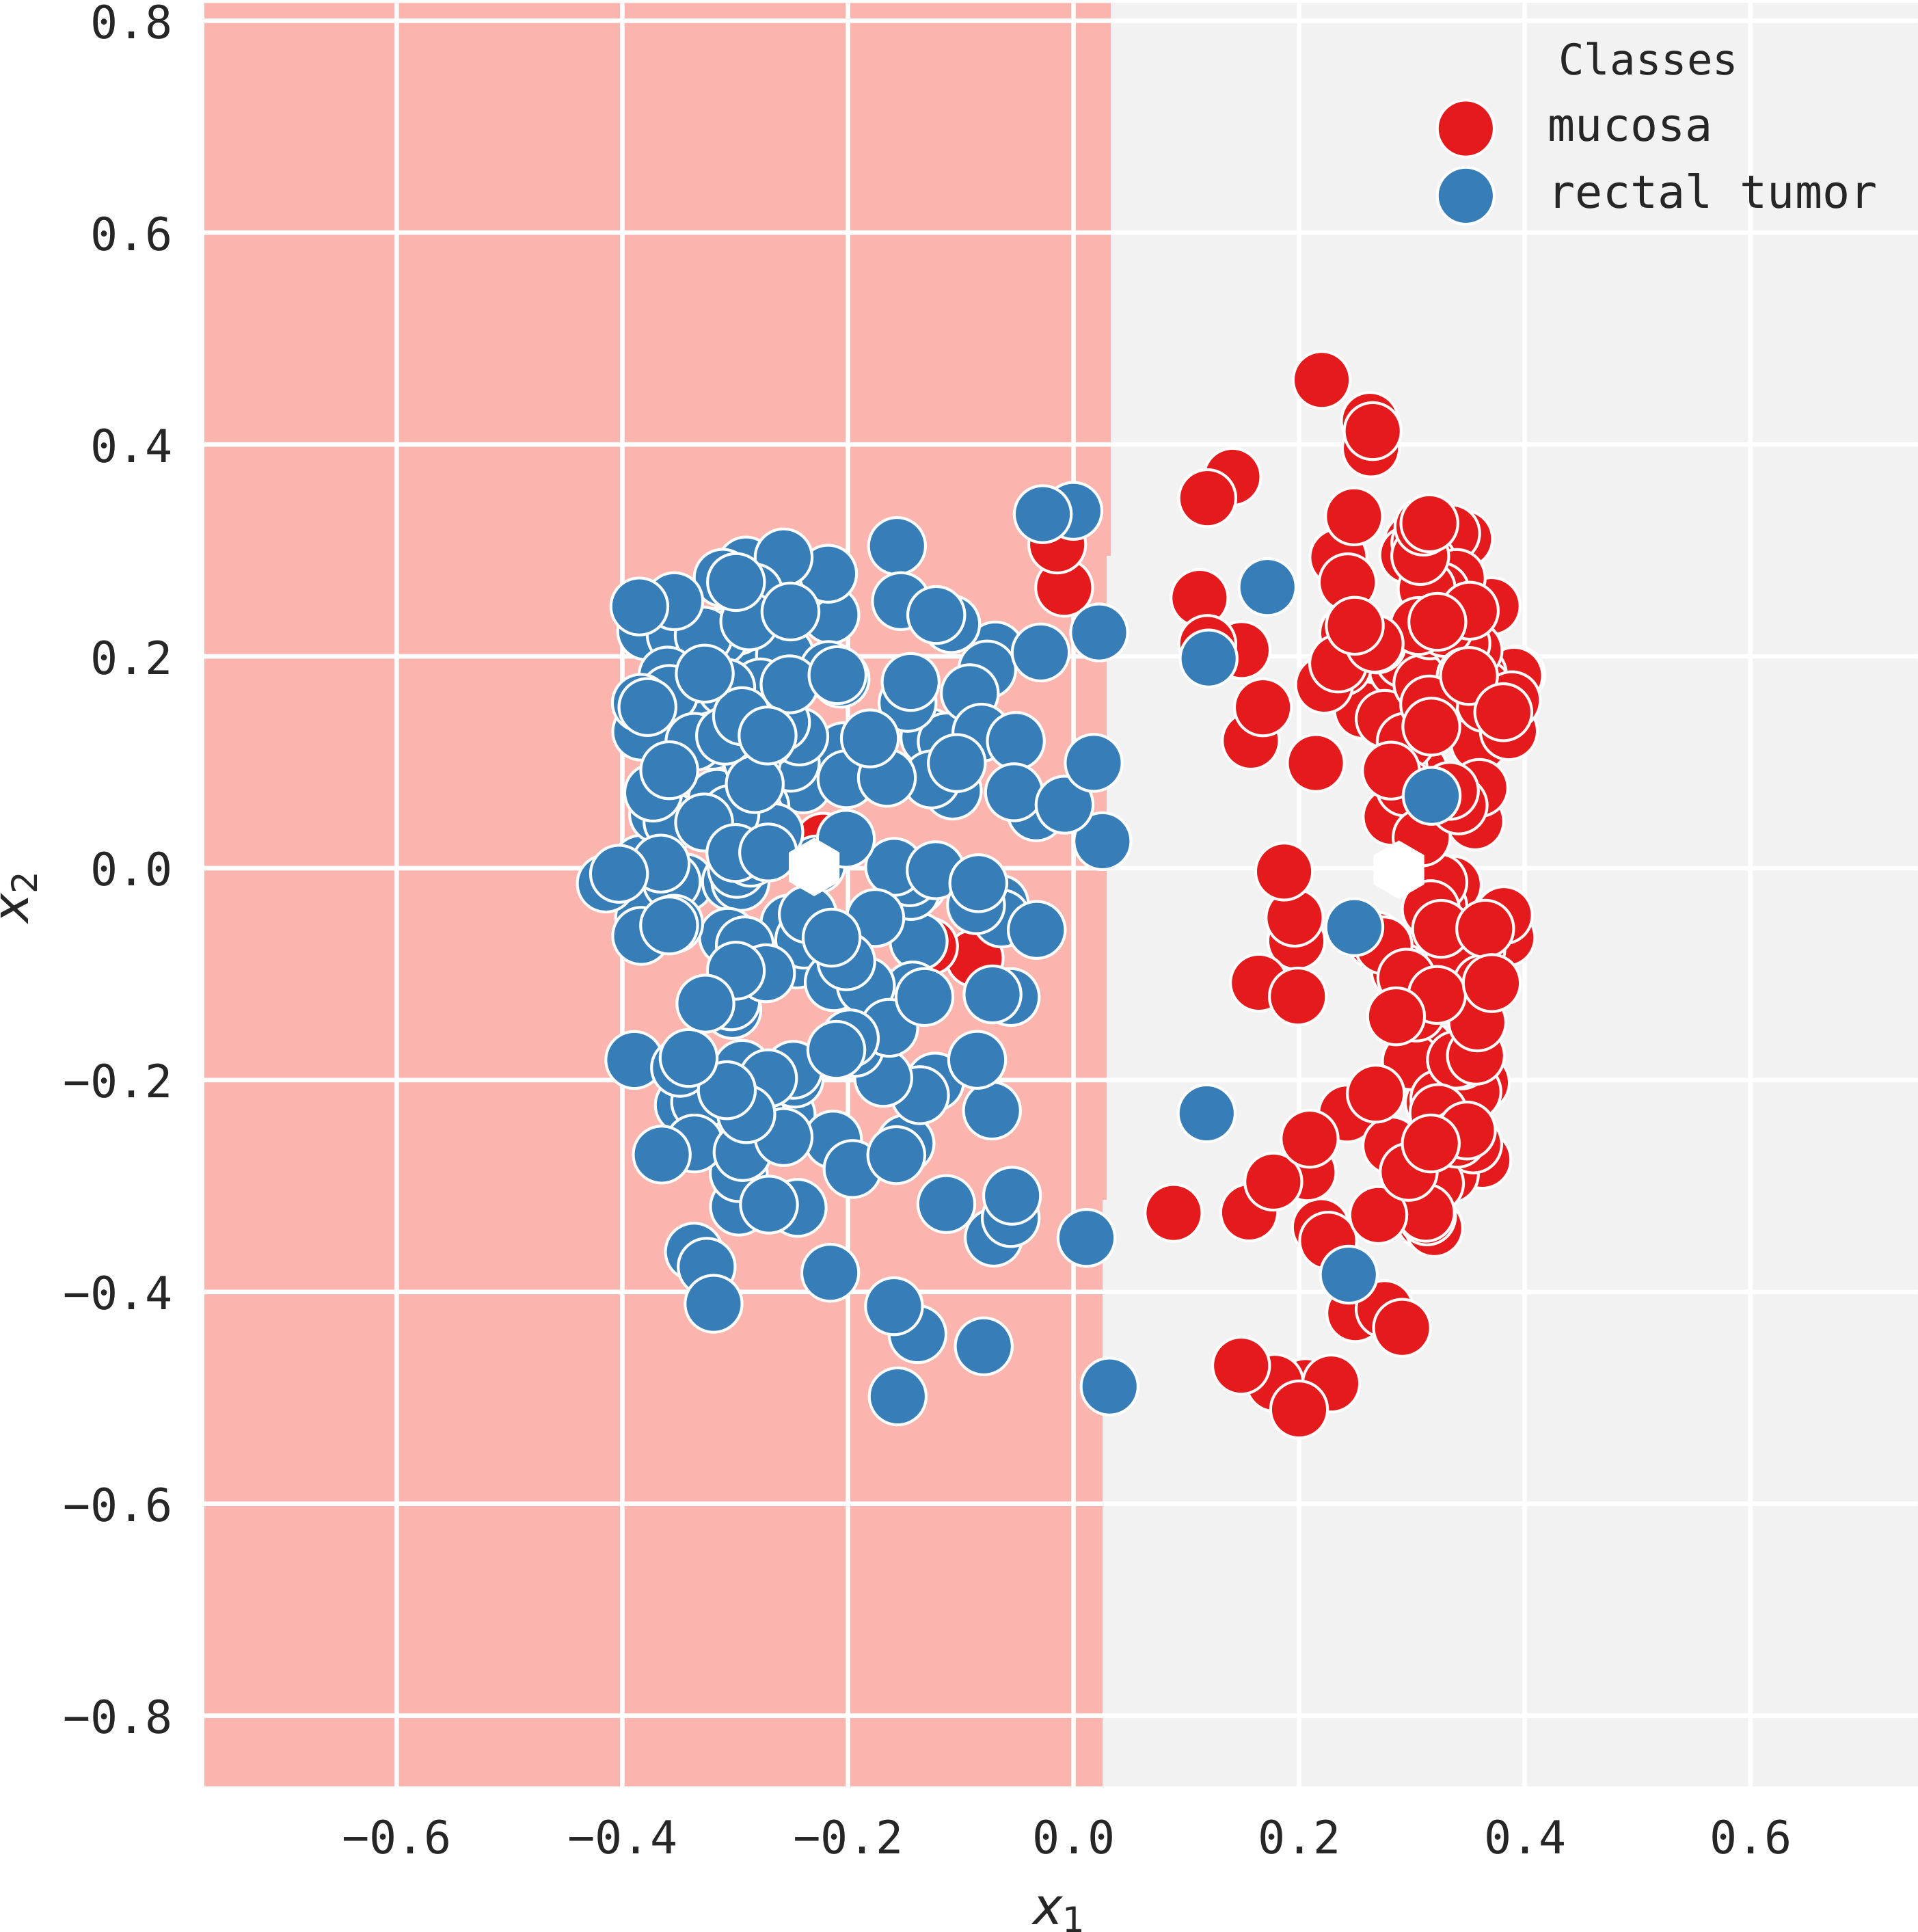
\includegraphics[width=0.32\textwidth]{part2/KMeans_2-clusts_rbf.png}
        \label{fig:b}%
    }%
    \hfill%
    \subfloat[]{%
        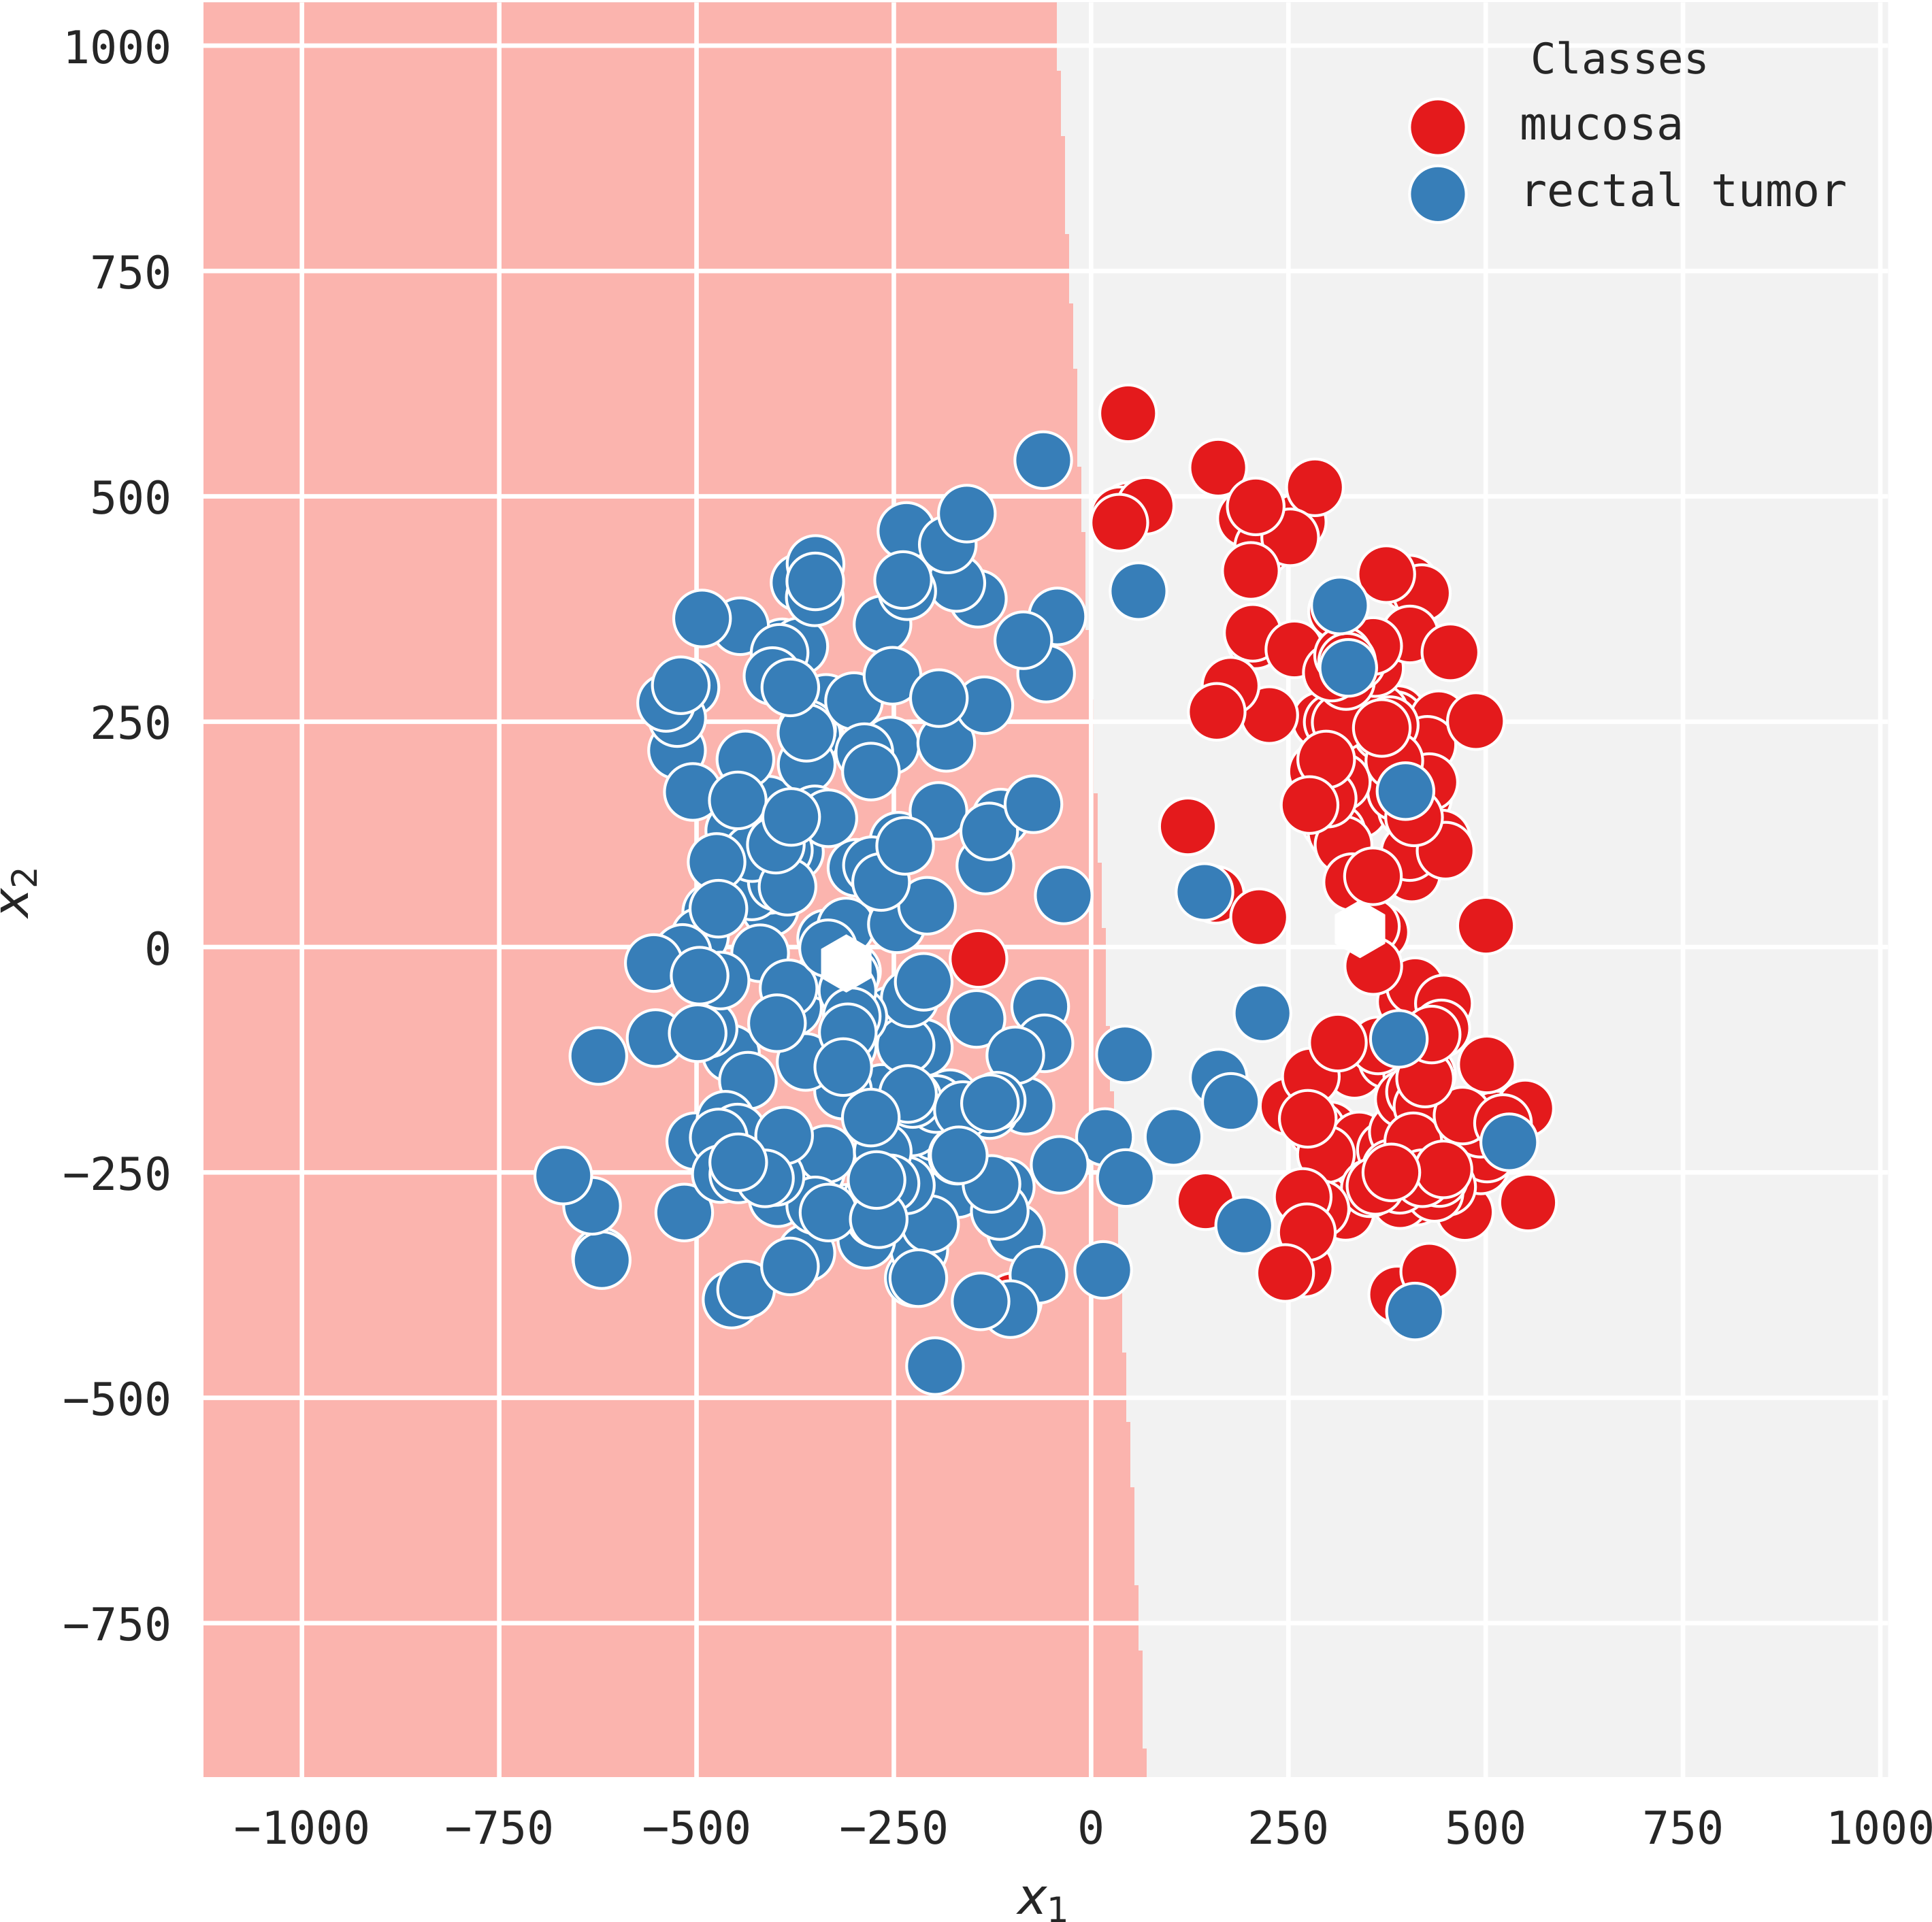
\includegraphics[width=0.32\textwidth]{part2/KMeans_2-clusts_isomap.png}
        \label{fig:c}%
    }%
    \caption{Three different 2D projections of the samples of the GEO gene expression data set used in this work. Projections on the left (a), middle (b) and right (c) panes are obtained via linear PCA, Gaussian PCA and isomap, respectively. The color of each point corresponds to the actual tissue type, while the background color is automatically learned by the $k$-means clustering algorithm. White hexagons correspond to cluster centroids.}\label{fig:scatter}
\end{figure}

For the second EDA, the relationships among the probe sets corresponding to the genes of the signature are separately explored learning a different hierarchical clustering~\cite{hastie2009elements} tree for mucosa (Figures~\ref{fig:mucosatree}) and CRC samples (Figure~\ref{fig:tumortree}), separately.
% shows some differences but some similarities too. This is easy explained by the fact that the mucosa samples derive from the same subjects from which the CRC samples are taken.
% The most evident similarities between these graphs are the following:
% such genes are also closely connected to TP53 and its isoform.
% and GSK3B-MSH2.1
The two trees are learned from different tissues, nevertheless they show some remarkable similarities. For instance, the pairs \tp-\tp{\small .1} and \msh-\pms{\small .1} always share a common parent. Interestingly, the first is a relationship between probe sets of the same gene, and the second is confirmed in literature, as \msh and \pms are both involved in hereditary non-polyposis CRC, a syndrome that predisposes for CRC.
Moreover, two probe sets of the the genes of \emph{S1}, namely \apc and \ctnnb, are consistently close to the root of the two trees. This suggest that the expression level of these two genes highly differs from the others.
% An interesting difference is the position of APC and CTNNB1 with respect to TP53 and its isoform. While in the CRC tree (Figure~\ref{fig:tumortree}) they
% it is evident that there is a direction in the connections of these genes (\ie the first gene is APC, the second is CTNNB1 and the last is TP53 with its isoform) this is not the case for the mucosa tree.
% The position of KRAS with respect to APC and CTNNB1 is another difference that emerges from the comparison of the two graphs: while in the CRC case, KRAS and KRAS.1 are located more or less on the same level in the middle of the graph, the reciprocal position of these two genes is quite different in the mucosa graph. KRAS is positioned close to the bottom of the graph while KRAS.1 is above KRAS and looks quite distant from it.
Two interesting differences between the two trees can also be noticed. First, most of the elements of the sublist \emph{S3}, which contains genes that enhance the risk of developing CRC, tend to be grouped together in Figure~\ref{fig:tumortree}, while the same observation cannot be done for Figure~\ref{fig:mucosatree}. Secondly, probe sets of the genes belonging to sublists \emph{S2} and \emph{S3} tend more to more closely connected in Figure~\ref{fig:tumortree} than in Figure~\ref{fig:mucosatree}.

% The Pearson correlations calculated among all the couples of the considered gene signature, produced two heatmaps one for each tissue type (see Figures XX and XX). From the comparison of these plots it is evident that there is a higher correlation in mucosa with respect to cancer tissue. We expected a clear difference in the appearance of the two heatmaps and the higher correlation in the mucosa samples could be related with the fact that the majority of these samples, disease-free, comes from the same subjects from which the cancer samples are retrieved. Therefore several genes of the signatures looks arelady altered in the mucosa while the same alteration in the tumor is not visible any more because the occurrence of many chromosomal aberrations (e.g., chromosomal translocation, inversions, deletion, gene mutations) it is expected to take place.

\begin{figure}[h!]
    \centering
    \subfloat[]{%
        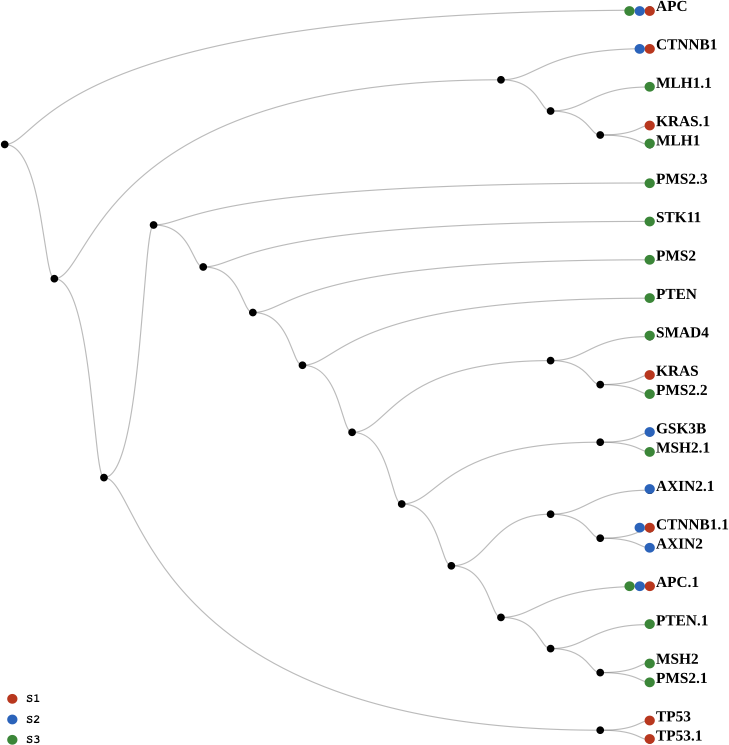
\includegraphics[width=0.45\textwidth]{part2/mucosa_tree_color.png}%
        \label{fig:mucosatree}%
    }%
    \hfill%
    \subfloat[]{%
        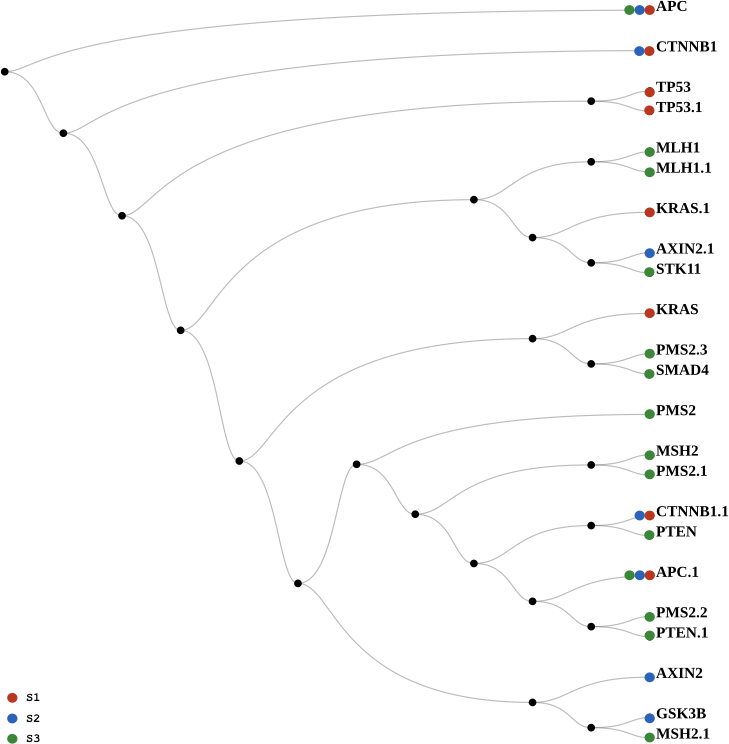
\includegraphics[width=0.45\textwidth]{part2/tumor_tree_color.png}%
        \label{fig:tumortree}%
    }%
    \caption{An example of hierarchical trees visualization learned by two \ade pipelines on mucosa (a) and CRC (b) samples. Each probe set is color coded according to the corresponding sublist. This visualization provides insights on the underlying structure of the measured gene expression level.}\label{fig:trees}
\end{figure}

% Please add the following required packages to your document preamble:
% \usepackage{booktabs}
% \begin{table}[]
%   \footnotesize
% \centering
% \caption{Perfomance summary of the three top performing \ade pipelines. The three pipelines only differ in the dimensionality reduction strategy. {\sl Pipe-1}, {\sl Pipe-2} and {\sl Pipe-3} resort to PCA, Isomap and Gaussian Kernel PCA, respectively}
% \label{tab:performance}
% \begin{tabular}{@{}lrrrr@{}}
% \toprule
% {\bf Pipeline}         & {\bf AMI}             & {\bf Completeness}    & {\bf Homogeneity}     & {\bf Silhouette} \\ \midrule
% \multicolumn{1}{l|}{\sl Pipe-1} & \multicolumn{1}{r|}{0.602} & \multicolumn{1}{r|}{0.603} & \multicolumn{1}{r|}{0.609} & 0.484                 \\
% \multicolumn{1}{l|}{\sl Pipe-2} & \multicolumn{1}{r|}{0.602} & \multicolumn{1}{r|}{0.603} & \multicolumn{1}{r|}{0.608} & 0.555                 \\
% \multicolumn{1}{l|}{\sl Pipe-3} & \multicolumn{1}{r|}{0.565} & \multicolumn{1}{r|}{0.566} & \multicolumn{1}{r|}{0.566} & 0.518 \\
% \bottomrule
% \end{tabular}
% \end{table}

% Pipe1
% median Impute-NaN $\to$ Recenter $\to$ linear KernelPCA $\to$ 2-clusts KMeans
% Pipe2
% median Impute-NaN $\to$ Recenter $\to$ Isomap $\to$ 2-clusts KMeans
% Pip3
% median Impute-NaN $\to$ Recenter $\to$ rbf KernelPCA $\to$ 2-clusts KMeans

\todo{...}
In this paper we presented \ade, a biomedical data exploration and visualization tool that can seamlessly run on single workstations as well as on HPC clusters.
Thanks to its scalable architecture, \ade is suitable for the analysis of large and high-dimensional data collections, that are nowadays ubiquitous in biomedicine.

\ade natively supports the integration with the GEO repository. Therefore, a user provided with the accession number of the data set of interest can select target phenotypes and genotypes and \ade takes care of automatically downloading the data and plugging them into the computational framework.
\ade offers a wide range of missing values imputing, data preprocessing, dimensionality reduction and clustering techniques that can be easily selected and applied to any input data.

In this paper we showed \ade capabilities performing two EDAs on a CRC gene expression data set. From the obtained results we can observe that a clear discrimination between CRC and control samples can be achieved by unsupervised data analysis pipeline.
% \apc and \ctnnb,
Moreover, a meaningful description of the relationships among the group of genes strongly associated with CRC can be represented as hierarchical trees.
